\documentclass[11pt]{beamer}
\usetheme{Dresden}
%\usecolortheme{beaver}
\usepackage[utf8]{inputenc}
\usepackage{amsmath}
\usepackage{amsfonts}
\usepackage{amssymb}
\usepackage{graphicx}
\usepackage{verbatim}
\author{NCC Moore}
\title{Topic 3 - Introduction to C}
%\setbeamercovered{transparent} 
%\setbeamertemplate{navigation symbols}{} 
%\logo{} 
\institute{McMaster University} 
\date{Summer 2021} 
\subject{COMPSCI 1XC3 - Computer Science Practice and Experience:
Development Basics} 
\stepcounter{section}

\definecolor{eggplant}{rgb}{0.5, 0.25, 0.5} % UBC Blue (primary)

\usecolortheme[named=eggplant]{structure}

\begin{document}

\begin{frame}
\center
COMPSCI 1XC3 - Computer Science Practice and Experience:
Development Basics
\titlepage
Adapted from C: How to Program 8th ed., Deitel \& Deitel
\end{frame}

\begin{frame}
\tableofcontents
\end{frame}

\section[Intro]{Thinking in C}
\begin{frame}{Hardware Vs Software}
\begin{itemize}
\item \textbf{Hardware} is a collection of physical, electronic components that comprise a computer's physical form.
\item \textbf{Software} is a series of instructions stored in a computer's memory that may be executed by sometimes arbitrary software systems.  
\item A processor is a group of circuits that implement operations on memory.
\item These operations are known as \textbf{instructions} or \textbf{hardware instructions}.
\end{itemize}
\end{frame}

\begin{frame}{Hardware Vs Software (cont.)}
Programming languages are more or less abstract, depending on how directly they access a system's underlying hardware.  
\begin{itemize}
\item In \textbf{High Level Languages} such as Python and Haskell, an operation may represent many hardware instructions.
\item In \textbf{Low Level Lanugages} such as C, an operation represents comparatively few hardware instructions.  
\end{itemize}
Different languages are good for different things, and a good developer knows which languages are suited to which applications! 
\end{frame}

\begin{frame}{So Why Learn a Low Level Language?}
\begin{itemize}
\item \textbf{Applications!} Anywhere you are programming close to the bare metal, you will probably be programming in C.  This includes:
\begin{itemize}
\item Operating Systems 
\item Kernels
\item Stuff you'll learn about in \emph{COMPSCI 2GA3 - Computer Architecture}
\end{itemize}
\item \textbf{Optimization!} Because they use a small number of hardware instructions per operation, programs written for low level languages can be very small, and run very quickly relative to high level languages.  Some optimizations are not possible in high level languages! 
\item \textbf{Knowledge!}  An appreciation for what our programs are doing ``under the hood'' will make us better programmers!  
\end{itemize}
\end{frame}

\begin{frame}{Von Neumann Architecture}
\center
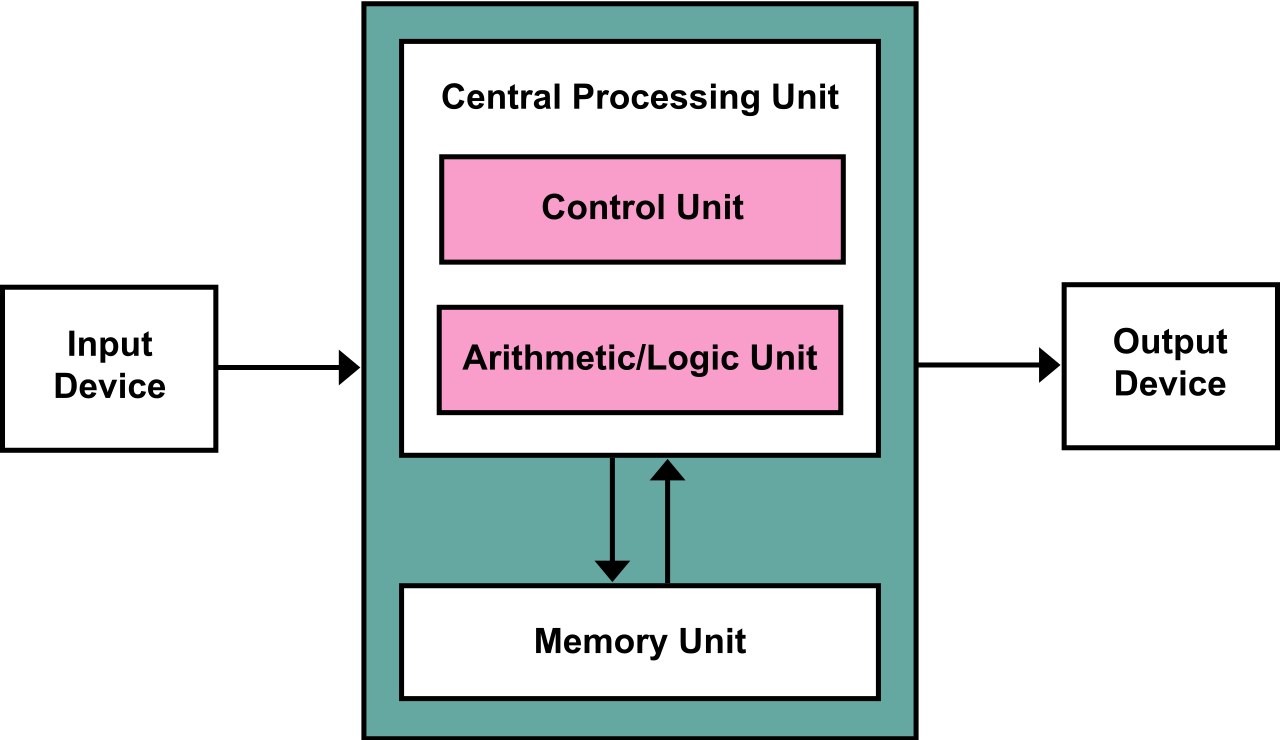
\includegraphics[scale=0.2]{VonNeumann.png}
\end{frame}

\section[C]{The C Programming Language}
\begin{frame}{The C Programming Language}
C evolved from two previous languages, BCPL and B.
\begin{itemize}
\item \textbf{BCPL} ("Basic Combined Programming Language") was developed in 1967 by Martin Richards as a language for writing operating-systems and compilers.
\item Ken Thompson modeled many features of his B language after their counterparts in BCPL, and in 1970 he used B to create early versions of the UNIX operating system at Bell Laboratories.
\end{itemize}
\end{frame}

\begin{frame}{The C Programming Language cont.}
\begin{itemize}
\item Dennis Ritchie at Bell Laboratories created the C language as an evolution of B in 1972.
\item C initially became widely known as the development language of the UNIX operating system.
\item Many of today's leading operating systems are written in C and/or C$++$. 
\begin{itemize}
\item The Windows, Linux, OS X, Android and iOS Kernels are all written mostly in C!
\end{itemize}
\item C is (mostly) hardware independent.
\item With careful design, it’s possible to write C programs that are portable to most computers. 
\end{itemize}
\end{frame}

\begin{frame}{Applications of C}
Because of it's high performance characteristics, C is still used a lot, despite being 50 years old! 
\begin{itemize}
\item \textbf{Operating Systems} - Portability across many hardware implementations and overall performance lend C to operating system development.  
\begin{itemize}
\item Linux, portions of Windows and Android use C
\item Apple's OS X uses Objective-C, which is derived from C.
\end{itemize} 
\item \textbf{Embedded Systems} - C is one of the most popular languages for embedded systems development, which are typically highly memory conservative.  
\end{itemize}
\end{frame}

\begin{frame}{Applications of C cont.}
\begin{itemize}
\item \textbf{Real-Time Systems} These ``mission critical'' applications require very fast response times.  A high performance language dramatically increases the feasibility of meeting timing constraints.
\item \textbf{Communication Systems} Due to the massive quantities of data being routed, optimization becomes crucial.  
\end{itemize}
\end{frame}

\begin{frame}{Popularity of C}
\center
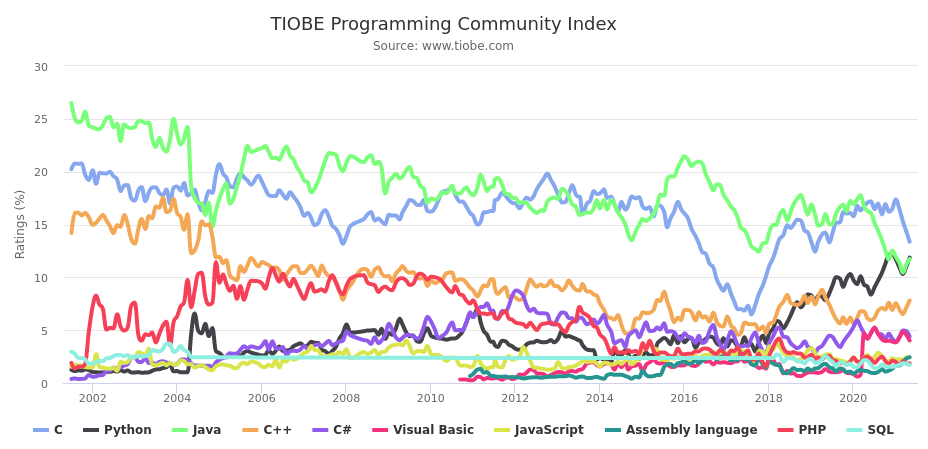
\includegraphics[scale=0.31]{tiobe.png} \\
As of May 2021, C is the world's most popular programming language according to the TIOBE index (\url{https://www.tiobe.com/tiobe-index/})
\end{frame}

\begin{frame}{Standards and Implementations}
The semantics of the C language are set by the International Standards Organisation (ISO) and the International Electrotechnical Commission (IEC), in a series of standard documents
\begin{itemize}
\item \textbf{C17} - ISO/IEC 9899:2018 (https://www.iso.org/standard/74528.html) is the latest version (June 2018).
\end{itemize}
There are many C compilers, which are all implementations of the above standard.  The following compilers are compliant with the latest version of the standard:
\begin{itemize}
\item GCC 8.1.0 
\item LLVM Clang 7.0.0
\item IAR EWARM v8.40.1
\end{itemize}
\end{frame}

\begin{frame}{The C Standard Library}
Because it lacks object oriented structures, the fundamental unit of abstraction in C is the \textbf{function}. 
\begin{itemize}
\item The most commonly used functions are collected into the \textbf{C Standard Library}.
\item Documentation may be found here: \url{https://www.gnu.org/software/libc/manual/pdf/libc.pdf}
\item Use of library functions is strongly encouraged!  
\item Library functions (especially from venerable libraries) have had \emph{decades} of optimization and improvement!  
\item Rule 1: If a library function exists, use it.
\item Rule 2: Learn Rule 1 quickly.  
\end{itemize}
\end{frame}

\section[C-Based Languages]{Other C-Based Languages}
\begin{frame}{C$++$}
C has been extremely influential on the development of many programming languages.  Perhaps C$++$ most obviously.
\begin{itemize} 
\item C$++$ was developed by Bjarne Stroustrup at Bell Laboratories.
\item It is an iterative improvement on C, crucially adding support for \textbf{object-oriented programming} (which C doesn't have!)
\item Object Oriented design adds the \textbf{object}, a new unit of abstraction that allows the combination of data with functions.
\item This increases modularization, and facilitates programming principals which allow very large programms to still be manageable.
\item We will not be studying C$++$ in this course.
\end{itemize}
\end{frame}

\begin{frame}{Other C-Based Languages} 
\begin{itemize}
\item \textbf{Objective-C} - An object-oriented language developed in the early 80s and eventually acquired by Apple.
\item \textbf{Java} - A C++ derived language developed by Sun Microsystems in 1991.  Uses the ``Java Virtual Machine'' to extend portability to a massive number of highly diverse systems and architectures.  Also, Minecraft.  
\item \textbf{C\#} - Microsoft's .net framework integrates internet connectivity into a framework of both Java and C$++$.  Non-Microsoft implementations of C\# also exist (such as game object scripting in the Unity game engine).
\end{itemize}
\end{frame}

\begin{frame}{Other C-Based Languages cont.}
\begin{itemize}
\item \textbf{PHP} - an object-oriented, open source scripting language used primarily in internet, database, and internet database applications.
\item \textbf{Python} (!) - Released in 1991 and developed by Guido van Rossum, python emphasizes the elimination of superfluous syntactic detail, and has become a very popular language for introductory programming courses.
\item \textbf{JavaScript} - The most widely used scripting language.  Adds dynamic behaviour to web pages.  
\end{itemize}
\end{frame}

\begin{frame}{Java is to JavaScript as Car is to Carpet}
\center
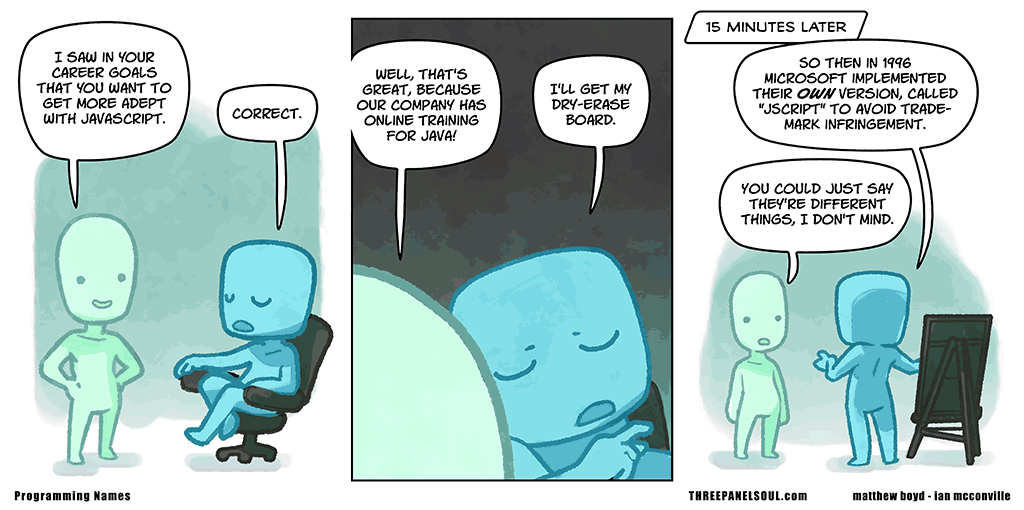
\includegraphics[scale=0.3]{javascript.png}
\end{frame}

\section[Working with C]{Working with C}
\begin{frame}{So compilers then...}
In contrast to the Python we all know and love from 1MD3, C is a \textbf{compiled}, rather than an \textbf{interpretted} language.  The process is as follows: 
\begin{enumerate}
\item editing
\item preprocessing
\item parsing
\item assembly
\item linking
\item loading 
\item executing
\end{enumerate}
\end{frame}

\begin{frame}{Editing a C file}
\begin{itemize}
\item C files may be edited using any text editor.  Common text editors include:
	\begin{itemize}
	\item Notepad / Notepad++ (Windows)
	\item Emacs / Gedit / Vim (Linux)
	\item TextEdit (Macintosh)
	\end{itemize}
\item Fancier environments (such as Jupyter and VS Code) allow for compilation and execution of C programs within the editor itself.
\item C files are given the *.c file extension
\item C header files (which we'll get to) have the *.h extension 
\end{itemize}
\end{frame}

\begin{frame}[fragile=singleslide]{Invoking the C Compiler}
The following process describes compiling a C program from the command line in a Linux-like environment.

Let's examine the following C file:
  
\hrule
\begin{verbatim}
#include<stdio.h>

int main () {
    printf("Hello, World!\n");
    return 0;
}
\end{verbatim}
\hrule
\end{frame}

\begin{frame}[fragile=singleslide]{Invoking the C Compiler cont.}
To compile this program, we use the following command in bash:
\begin{verbatim}
[...]$ gcc simple.c -o simple
\end{verbatim}
\begin{itemize}
\item First, we invoke gcc, the gnu compiler collection.  gcc knows we want to interpret the file as a C program because of the file extension.
\item Next, we specify the file to be compiled.  
\item the \texttt{-o} flag allows us to specify the name of the produced executable file.  
\item The produced file is the original program expressed in machine language (also known as \textbf{object code}).  Note that this is different from assembly language!  
\end{itemize}
\end{frame}

\begin{frame}{The Compilation Process}
Once the compiler is invoked, it goes through a couple stages:
\begin{itemize}
\item \textbf{Preprocessing} - The purpose here is to make the code ready for parsing and generation.
\begin{itemize}
\item Removing comments
\item Expanding any Macros
\item Expanding any included code (``include'' in C is equivalent to ``import'' in Python) 
\item A few other things
\end{itemize} 
\item \textbf{Parsing} - The code is broken down into \textbf{tokens} (also known as tokenization).  The tokens are arranged into a hierarchical \textbf{Abstract Syntax Tree} (AST).
\item \textbf{Assembly} - The AST is used to create a series of machine code instructions, which are saved as an object file (*.o)
\item \textbf{Linking} - The object file is linked up with the relevant libraries, and an executable is produced.  
\end{itemize}
\end{frame}

\begin{frame}{The Compilation Process cont.}
\center
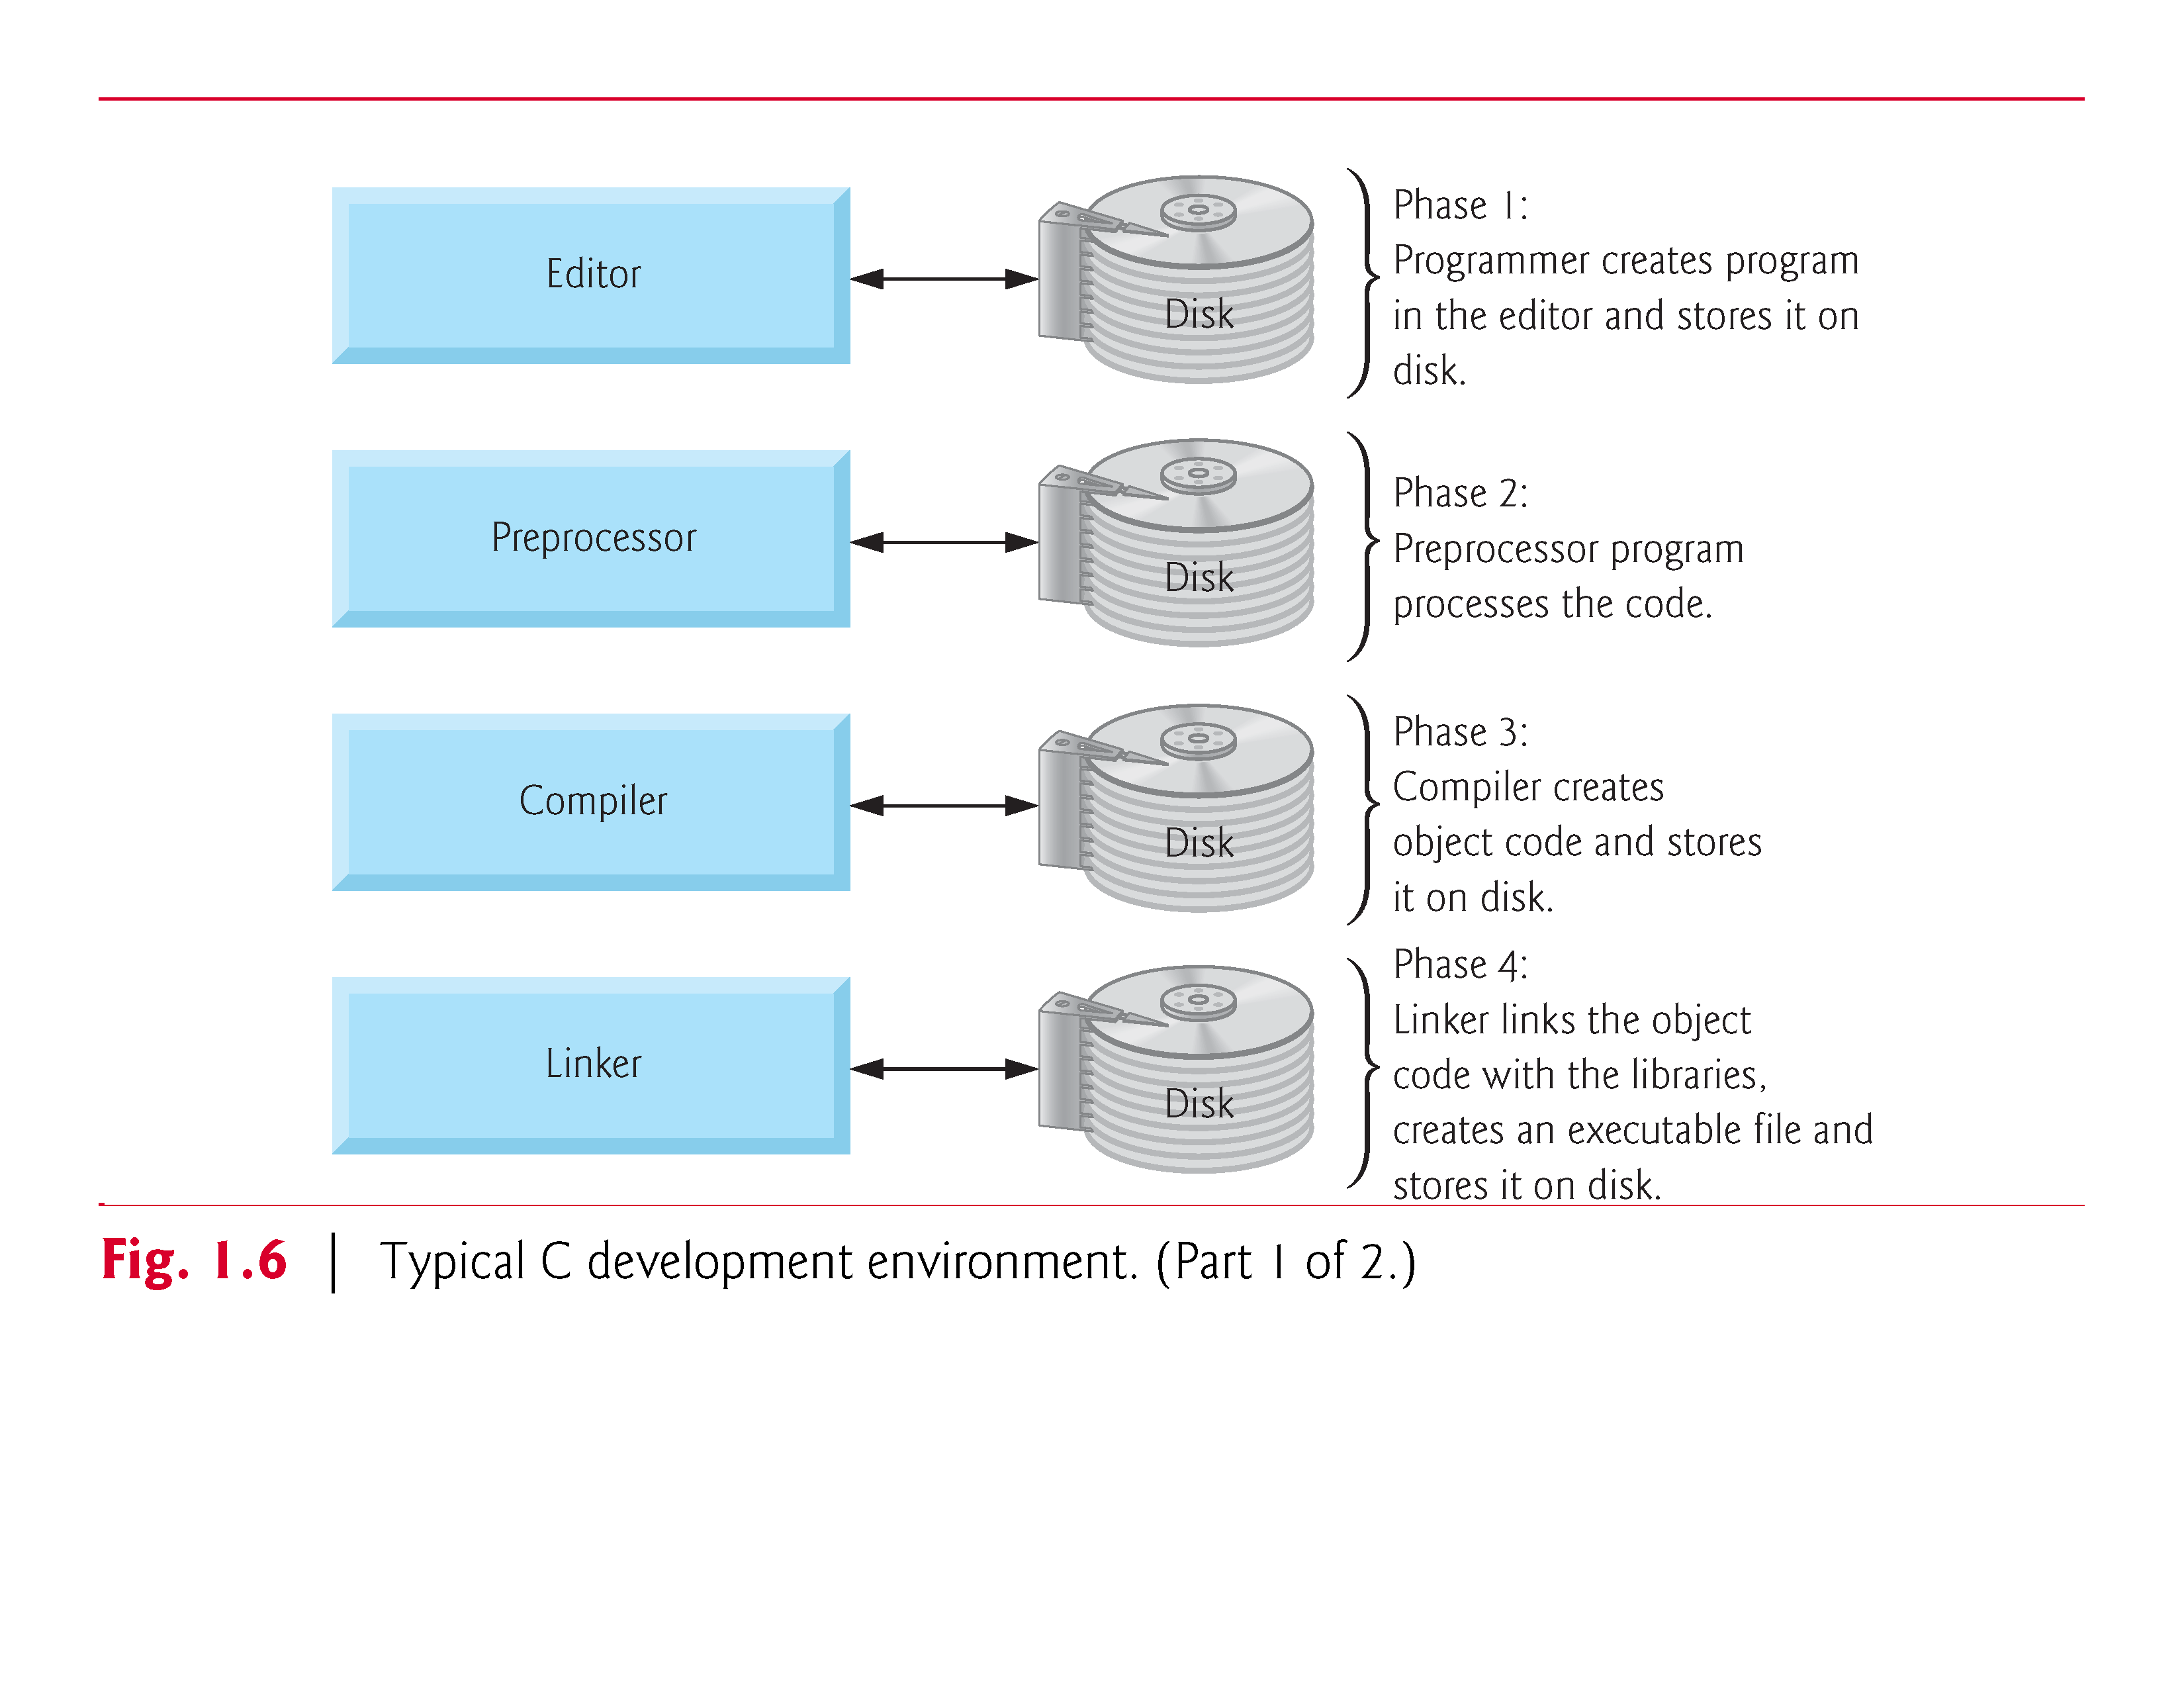
\includegraphics[scale=0.35]{compile.png}
\end{frame}

\begin{frame}{Compiler Complaints!}
Your invokation of gcc may not end successfully, if your code has bugs in it! 
\begin{itemize}
\item \textbf{Syntax Errors} occur during parsing, if the code can not be parsed correctly
	\begin{itemize}
	\item For example, forgetting a semicolon causes a Syntax Error
	\end{itemize}
\item \textbf{Compiler Warnings} do not halt execution of the compiler, but they can indicate other problems with your code.  
	\begin{itemize}
	\item Some warnings are not shown by default, but the \texttt{-Wall} (Warnings: All) flag tells gcc you want to see them.
	\item If you don't want to see any warnings (not recommended...), use the \texttt{-w} flag.
	\item You may be warned about:
		\begin{itemize}
			\item Using data types and pointers incorrectly
			\item Not using variables that have been declared
			\item Using \texttt{=} instead of \texttt{==}
		\end{itemize}
	\end{itemize}
\end{itemize}
\end{frame}

\begin{frame}[fragile=singleslide]{Executing the Executable}
In a Linux-like environment, an executable is run using the following command:
\begin{verbatim}
[...]$ ./simple
\end{verbatim}
\begin{itemize}
\item \textbf{Loading} - The compiled C program is loaded into the system's primary memory (usually the RAM)
\item \textbf{Execution} - The CPU runs the program, starting with the first instruction, and proceeding until the program terminates.  
\end{itemize}
\end{frame}

\begin{frame}{Executing the Executable cont.}
\center
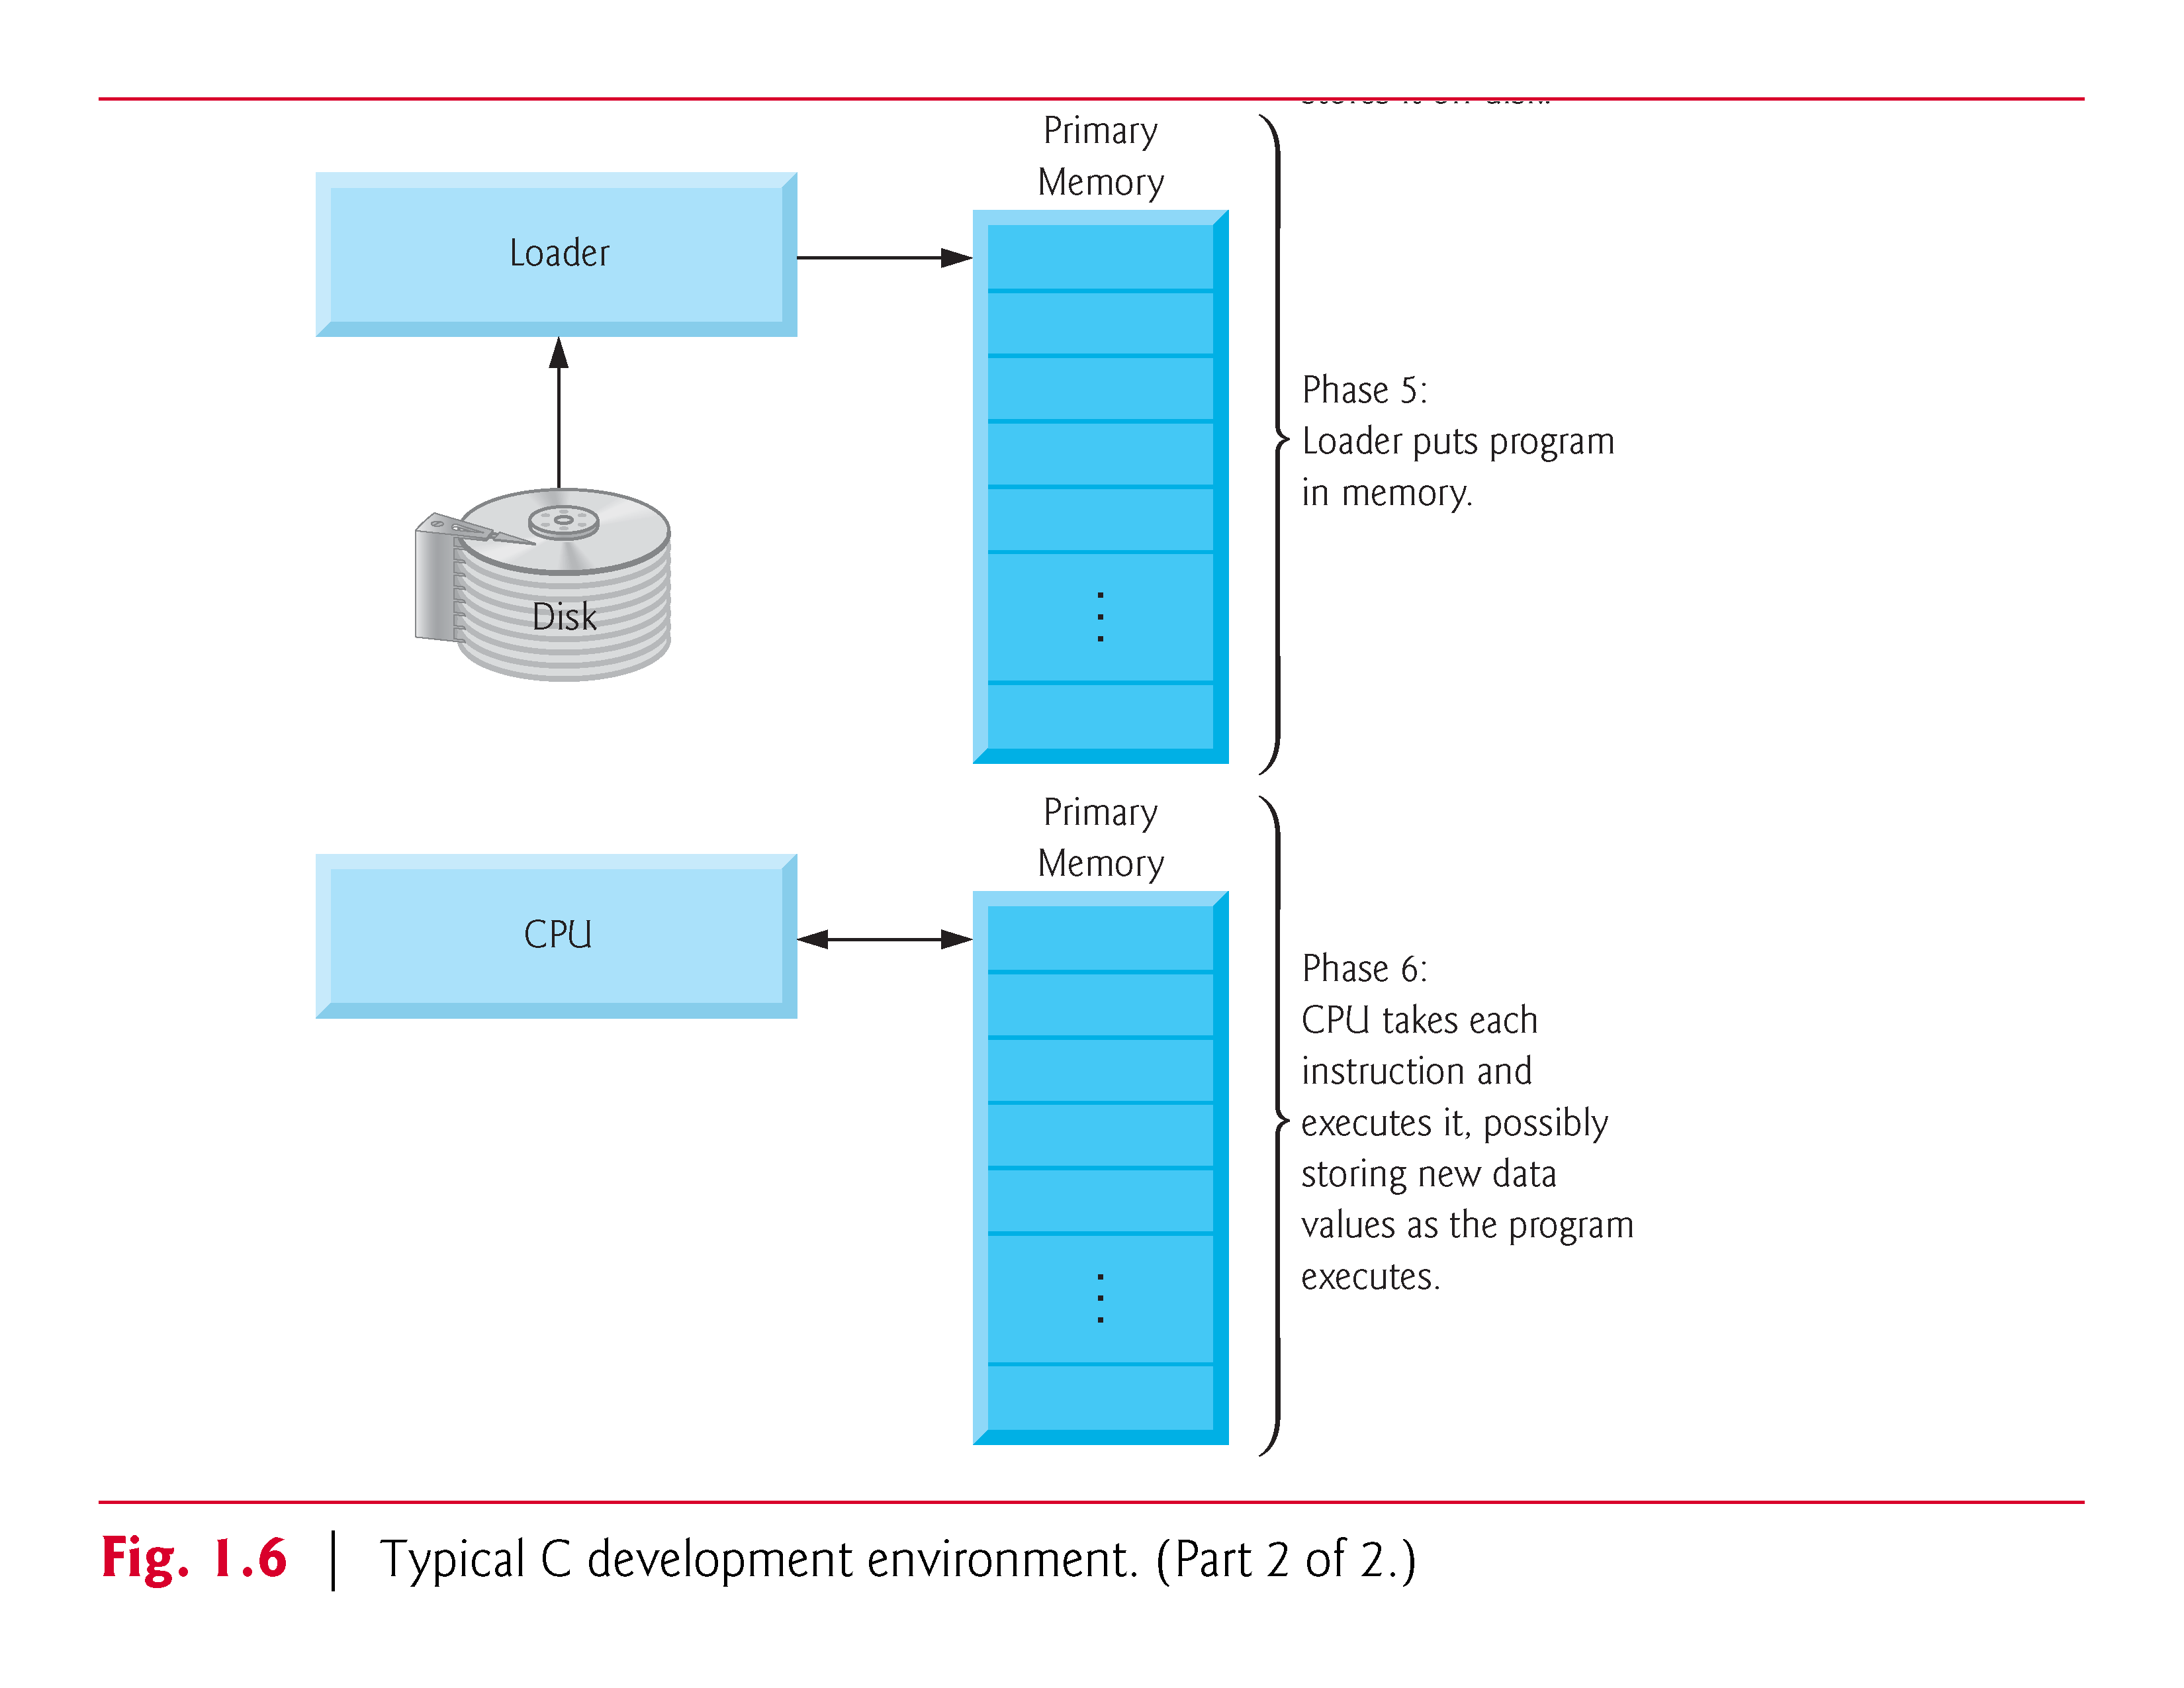
\includegraphics[scale=0.35]{execute.png}
\end{frame}

\begin{frame}{When Runtime isn't Funtime}
Often, your code will contain bugs, despite being compiled and linked successfully.  These are known as \textbf{semantic} errors.
\begin{itemize}
\item Some semantic errors will just straight up crash your program. These are known as \textbf{fatal errors}.
	\begin{itemize}
	\item Dividing by Zero!
	\item Trying to access memory that doesn't belong to you! (The dreaded Segfault!)
	\end{itemize}
\item Others just cause a mismatch between the expected output of a program and it's actual output.  
	\begin{itemize}
	\item It is important to know what the expected result of a program is for specific inputs.
	\item Running a program with specific inputs and looking for a known ``correct'' output is known as \textbf{testing}.
	\end{itemize}
\end{itemize}
\end{frame}

\begin{frame}{Runtime Interactions}
If we wish to interact with a C program using a monitor and keyboard, that C program needs to interact with the following:
\begin{itemize}
\item \textbf{\texttt{stdin}} - (standard input stream) a place in your computer where keystrokes are logged for retrieval by programs.
\item \textbf{\texttt{stdout}} - (standard output stream) a place which collects things programs wish to print to the screen.  
\item \textbf{\texttt{stderr}} - (standard error stream) similar to stdout, but reserved specifically for error messages.  
\end{itemize}

All three of these streams are either \textbf{emulated} or are connected in a more complex manner in environments such as VS Code, but are used directly in bash-style environments.
\end{frame}

\begin{frame}{The Last Slide Comic}
\center
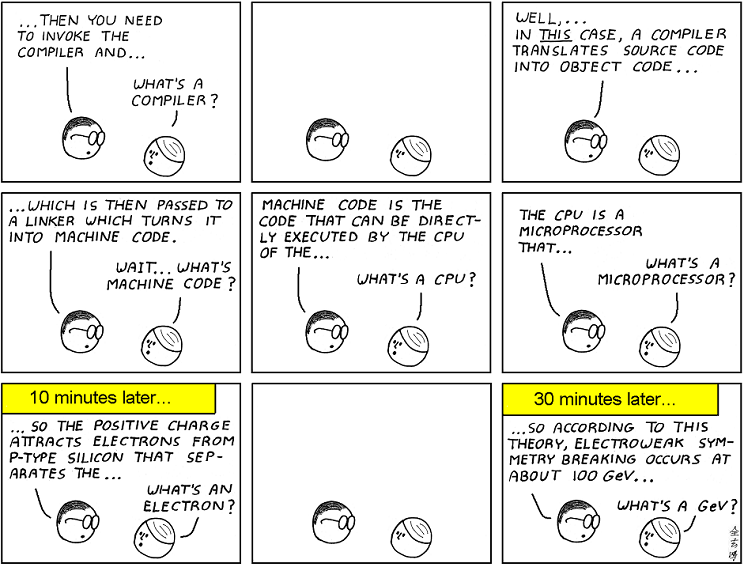
\includegraphics[scale=0.3]{CompilerComic.png}
\end{frame}

\end{document}